%    Programming in C
% notes:
%~~~~~~~~~
%-------------------------------------------------------------------------------------------------------------------------------------------
% file C.tex
%-------------------------------------------------------------------------------------------------------------------------------------------
% Setting path to image 
\graphicspath{{../src/C/img/}}

\lstset{ %
  language=C,                            % choose the language of the code
  basicstyle=\footnotesize,              % the size of the fonts that are used for the code
  backgroundcolor=\color{White},         % choose the background color. You must add \usepackage{color}
  commentstyle=\color{help}\textit,
  keywordstyle=\color{keyword}\textbf,
  breaklines=true,                       % sets automatic line breaking
  breakatwhitespace=true,                % sets if automatic breaks should only happen at whitespace
  showspaces=false,                      % show spaces adding particular underscores
  showstringspaces=true,                 % underline spaces within strings
  showtabs=true,                         % show tabs within strings adding particular underscores
  frame=none,	                           % adds a frame around the code - none, single
  tabsize=8,                             % sets default tabsize to 8 spaces
  captionpos=b,                          % sets the caption-position to bottom
  numbers=left,                          % where to put the line-numbers -none, left, right
  numberstyle=\footnotesize,             % the size of the fonts that are used for the line-numbers
  stepnumber=1,                          % the step between two line-numbers. If it's 1 each line
                                         % will be numbered
  xleftmargin=3em,                       % adjust left margin
}
%===================================== Kapitola: Terminálový vstup a výstup ============================================================
%==============================Kapitola: Terminálový vstup a výstup=======================================================  
\chapter{Terminálový vstup a výstup}
\minitoc
\newpage
  Jazyk C, narozdíl od Pascalu, nedefinuje žádnou \texttt{I/O (vstup\-ně/výstup\-ní -In\-put/Out\-put)} operaci jako část jazyka.
  Nezbytné vstupy a výstupy jsou řešeny tak, že standardní knihovna obsahuje několik funkcí, které \texttt{I/O} zajišťují.

  Nejvíce strojově závislé akce jsou I/O operace a tímto způsobem se tedy důsledně oddělují strojově závislé a strojově nezávislé
  části jazyka. Tato skutečnost je pak významným přínosem při vytváření kompilátoru pro jiný počítač.

  \begin{figure}[ht!]
     \centering
     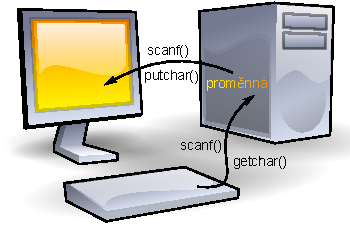
\includegraphics[scale=1.2]{terminalovy_IO_skica.pdf}
     \caption{Operace pro terminálový vstup a výstup}\label{C:fig_Terminal_IO}
  \end{figure}

  \section{Hlavičkový soubor \lstinline[basicstyle=\ttfamily]!stdio.h!}
    Aby bylo možno správně používat všechny funkce pro vstupu a výstupu, je nutné na začátku programu připojit "popis" těchto
    funkcí. Ten se nachází v hlavičkovém (\emph{header}) souboru \lstinline[basicstyle=\ttfamily]!stdio.h!:

    \lstinline[basicstyle=\ttfamily]!#include <stdio.h>  //zde neni strednik!

    Od tohoto okamžiku je pak možné používat dále popsané funkce.

  \section{Standardní vstup a výstup znaku}
    Výstup jednoho znaku zajišťuje \lstinline[basicstyle=\ttfamily]!putchar()! a vstup jednoho znaku funkce
    \lstinline[basicstyle=\ttfamily]!getchar()!.
    \begin{itemize}
      \item \lstinline[basicstyle=\ttfamily]!int putchar(int c);!
      \item \lstinline[basicstyle=\ttfamily]!int getchar(void);!
    \end{itemize}
    Obě funkce pracují s proměnnými \lstinline[basicstyle=\ttfamily]!int! a ne \lstinline[basicstyle=\ttfamily]!char!.

      \marginpar{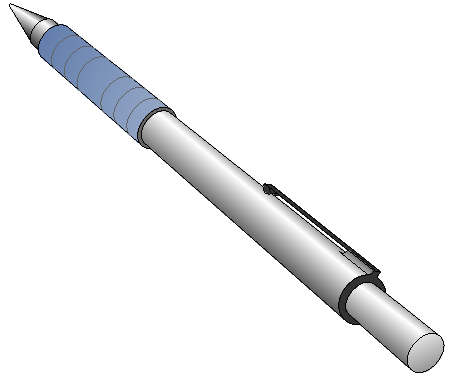
\includegraphics[width=0.09\textwidth]{pen.pdf}}
      %---------------------------------------------------------------
      \lstinputlisting{../src/C/file/Cteni_tisk_znaku.c} 
      \begin{lstlisting}[caption=\texttt{Cteni\_tisk\_znaku.c} Čtení a tisk znak ze standardního vstupu na standardní výstup.]
      \end{lstlisting}
      %--------------------------------------------------------------    
    
    \begin{example}Čtení znaku ze standardního vstupu a jejich zápis na standardní výstup ukazuje následující program,
      představující jednoduchou variantu příkazu kopírování souboru (nutno ovšem přesměrovat vstup a výstup).

      \marginpar{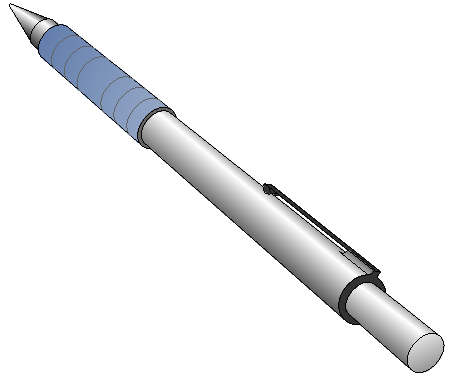
\includegraphics[width=0.09\textwidth]{pen.pdf}}
      %---------------------------------------------------------------
      \lstinputlisting{../src/C/file/CPY.c}
      \begin{lstlisting}[caption=\texttt{CPY.c} Kopíruje znak ze standardního vstupu na standardní výstup.]
      \end{lstlisting}
      %---------------------------------------------------------------
    \end{example}
    
  \section{Standardní vstup a výstup řetězců}
    Standardní vstup a výstup řetězců je jednoduchou nadstavbou nad čtením znaku. Obě funkce,
    \begin{itemize}
      \item \lstinline[basicstyle=\ttfamily]!char *gets(char *s);!
      \item \lstinline[basicstyle=\ttfamily]!int puts(const char *s);!
    \end{itemize}
    pracují s řetězci. \texttt{gets()} načte do znakového pole vstupní řetězec az do konce řádku, symbol
    \lstinline[basicstyle=\ttfamily]!'\n'! není do znakového pole zapsán. Ukazatel na pole (načtený řetězec) je rovněž návratovou
    hodnotou. Chybu signalizuje návrat NULL. \texttt{puts()} zapíše řetězec na výstup a přidá přechod na novy řádek
    \lstinline[basicstyle=\ttfamily]!'\n'!. Chybu představuje návratové \texttt{EOF}, jinak vrací kladné cele číslo.

    Jednoduchost použití skrývá velké nebezpečí. Funkce \texttt{gets()} nemá informaci o délce oblasti vymezené pro čtený
    řetězec. Je-li oblast kratší, než vstupní řádek, dojde jeho načtením velmi pravděpodobně k přepsání paměťové oblasti
    související s vyhrazenou pamětí. A to se všemi důsledky z toho vyplývajícími.


  \section{Formátovaný standardní vstup a vystup}
  \section{Souhrnné cvičení}
    \begin{example}Vytvořte program, který vygeneruje ASCII tabulku se čtyřmi sloupci ve formátu \textbf{[znak|kód|znak|kód]}.
      Rozsah tabulky definujte pomocí dvou symbolických konstant \lstinline[basicstyle=\ttfamily]!MIN_ASCII, MAX_ASCII!.

      \marginpar{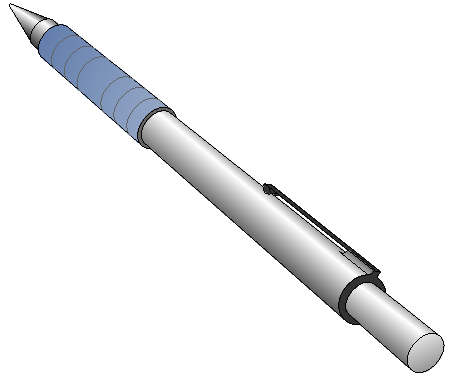
\includegraphics[width=0.09\textwidth]{pen.pdf}}
      %---------------------------------------------------------------
      \lstinputlisting{../src/C/file/ASCII.c}
      \begin{lstlisting}[caption=\texttt{ASCII.c} Generuje ASCII tabulku na terminálu.]
      \end{lstlisting}
      %---------------------------------------------------------------
    \end{example} 
%===================================== Kapitola: Pointery ===============================================================================
%======================================Kapitola: Pointery===============================================================  
\chapter{Pointery}
\minitoc
\newpage
  \textbf{Pointery} (též ukazatele nebo směrníky) jsou \emph{"srdce a duše jazyka C"}. Pointer je proměnná, jako každá jiná, pouze hodnota uložená v této proměnné má jiný význam. Pointer představuje \textit{adresu paměti} a na této adrese se teprve ukrývá příslušná hodnota. Pointer je tedy proměnná uchovávající paměťovou adresu.\cite{Herout}

  \section{Základy práce s pointery}
    \begin{figure}
      \centering
      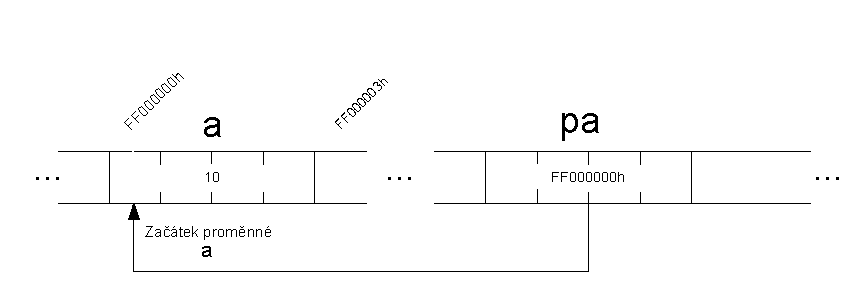
\includegraphics[width=135mm]{princip_ukazatele.pdf}
      \caption{Princip ukazatele v paměti}
      \label{figure:pointer1}
    \end{figure}
    \begin{example}Vytvořte funkce kopírující prvky jednoho pole do druhého pomocí indexu i ukazatele.
    
      \marginpar{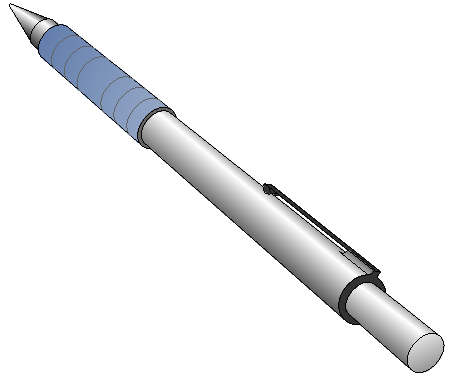
\includegraphics[width=0.09\textwidth]{pen.pdf}}    
      %---------------------------------------------------------------
      \lstinputlisting{../src/C/file/CPYARRY.C}
      \begin{lstlisting}[caption=\texttt{CPYARRY.C} Kopíruje prvky jednoho pole do druhého.]
      \end{lstlisting}
      %---------------------------------------------------------------
      Výstup programu:                                                     \newline
        \lstinline[basicstyle=\ttfamily]!1   2   3   4   5   6   7   8   9!\newline
        \lstinline[basicstyle=\ttfamily]!1   2   3   4   5   6!            \newline
        \lstinline[basicstyle=\ttfamily]!4   5   6   7   8   9!            \newline
    \end{example} 
%======================================Kapitola: Preprocesor jazyka C ===================================================================  
%======================================Kapitola: Preprocesor jazyka C ===================================================================  
\chapter{Preprocesor jazyka C}
\minitoc
\newpage
  Preprocesor interpretuje jednoduché direktivy pro vložení zdrojového kódu z jiného souboru (\lstinline[basicstyle=\ttfamily]!#include!), definice maker (\lstinline[basicstyle=\ttfamily]!#define!) a podmíněné vložení kódu (\lstinline[basicstyle=\ttfamily]!#if!).\texttt{C} preprocesor přijímá tyto direktivy:
  
  \begin{table}[ht!]
    \centering
    \begin{tabular}{c c c c}
      \hline
      \lstinline[basicstyle=\ttfamily]!#define! & \lstinline[basicstyle=\ttfamily]!#elif! & \lstinline[basicstyle=\ttfamily]!#else! & \lstinline[basicstyle=\ttfamily]!#endif! \\
      \lstinline[basicstyle=\ttfamily]!#error! & \lstinline[basicstyle=\ttfamily]!#if! & \lstinline[basicstyle=\ttfamily]!#ifdef! & \lstinline[basicstyle=\ttfamily]!#ifndef! \\
      \lstinline[basicstyle=\ttfamily]!#include! & \lstinline[basicstyle=\ttfamily]!#line! & \lstinline[basicstyle=\ttfamily]!#pragma! & \lstinline[basicstyle=\ttfamily]!#undef! \\
      \hline            
    \end{tabular}
    \caption{Seznam platných direktiv jazyka \texttt{C}}\label{S4101C1:C_tab_direktiva}
  \end{table} 
  
 \section{Připojení externích souborů}
 
 \section{Definice maker}
   Definice maker ve významu rozsahů polí je typickým příkladem použití preprocesoru. Ve zdrojovém textu se neodvoláváme na magická čísla, ale na vhodně symbolicky pojmenovaná makra, která zvýší čitelnost programu.

   Pro větší přehlednost rozdělme makra na 
   \begin{itemize}
     \item symbolické konstanty,
     \item makra
   \end{itemize}
   Klíčem nechť je skutečnost, že makro na rozdíl od symbolické konstanty má argumenty.
   \subsection{Symbolické konstanty}
   \subsection{Makra}   
   
 \section{Podmíněný překlad}  
   Preprocesor může během své činnosti vyhodnocovat, je-li nějaké makro definováno, či nikoliv. Při použití klíčového slova preprocesoru \texttt{defined} pak může spojovat taková vyhodnocení do rozsáhlejších logických výrazů. Argument defined nemusí být uzavřen do závorek. Může se však vyskytnout jen za \lstinline[basicstyle=\ttfamily]!#if! nebo \lstinline[basicstyle=\ttfamily]!#elif!. Například si ukažme složitější podmínku: